\documentclass[12pt, letterpaper]{article}

\usepackage{xspace}
\usepackage{amsmath} % has \nobreakdash
\usepackage{graphicx}
\usepackage[utf8]{inputenc}
\usepackage{booktabs}
\usepackage{hyperref}
\usepackage{aas_macros}

\usepackage[top=1in, bottom=1.5in, left=1in, right=1in]{geometry}

\graphicspath{{./figures/}}

\newcommand{\superk}  {Super\nobreakdash-K\xspace}

\title{Target of Opportunity proposal for locating a core collapse
  supernova in our galaxy triggered by a neutrino supernova alert}
\author{ C.W. Walter, D. Scolnic, A. Slosar}
\date{ November 2018}

\begin{document}

\maketitle

\begin{abstract}

  A few times a century, a core collapse supernova (CCSN) occurs in our
  galaxy. When such a core collapse supernova happens, over 99\%
  of its gravitational binding energy is released in the form of
  neutrinos.  Over a period of 10s of seconds a powerful neutrino flux
  is emitted from the collapsing star.  When the exploding shock wave
  finally reaches the surface of the star, optical photons escaping
  the expanding stellar envelope leave the star and eventually arrive at
  Earth as a visible brightening.

  By combining the multi-messenger signal from optical, neutrino, and
  gravitational waves, we afford an unprecedented opportunity to learn
  about the astrophysics of these rare objects. Carefully measuring
  the optical light curve of the explosion will give critical
  information about the size and composition of the progenitor star
  and help understand the dynamics of the explosion.

  Crucially, although the neutrino signal is prompt, the time to the
  shock wave breakout can be minutes to many hours later.  This means
  that the neutrino signal will serve as an alert, warning the
  optical astronomy community the light from the explosion is coming.  
  Quickly identifying the location of the supernova on the sky and
  disseminating it to the all available ground and spaced-based
  instruments will be critical to learn as much as possible about the
  event.

  Some neutrino experiments can report pointing information for these
  galactic CCSN. In particular, the Super-Kamiokande experiment can
  point to a few degrees for CCSN near the center of our galaxy.  A
  CCCN located 10~kpc from Earth is expected to result in a pointing
  resolution of the order of $3^\circ$.  LSST's field of view (FOV) is
  well matched to this initial search box.  LSSTs depth is also
  uniquely suited for identifying CCSN even if they fail or are
  obscured by the dust of the galactic plane.

  This is a proposal to, upon receipt of such an alert, use LSST for
 a full day of observing to continuously monitor a pre-identified
  piece of sky and, by using difference imaging, identify and announce
  the location of the supernova. In this proposal, we propose to use one
  night (approximately .03\% of the survey period) if a galactic
  supernova occurs.  Based on estimates of the rate of such CCSN there
  is approximately a 20\% chance that a CCSN will occur during the
  survey period.
  
\end{abstract}

\section{White Paper Information}

\noindent
Authors: \\

\noindent
Chris Walter - chris.walter@duke.edu \\
Dan Scolnic - dan.scolnic@duke.edu \\
Anze Slozar - anze@bnl.gov \\

\noindent
Categorization: 
\begin{enumerate} 
\item {\bf Science Category:}  Exploring the transient optical sky
\item {\bf Survey Type Category:}  Target of Opportunity observation
\item {\bf Observing Strategy Category:}  A single night, continuous
  observation strategy focused on one few degree field pointing as given by
  a neutrino supernova alert trigger.
\end{enumerate}  

\clearpage

\section{Scientific Motivation}
\label{sec:motivation}

No visible galactic CCSN have been seen and measured in the modern
scientific era.  Although the rate is not completely known, CCSN are
thought to occur roughly two or three times a century.  The closest
modern CCSN we have observed was SN1987a in the LMC.  Using a alarm
from neutrino detectors as a trigger, LSST can quickly identify and
characterize a galactic core-collapse supernova and then notify the
rest of the astronomical community which can then track it in multiple
wavelengths from the ground and space.  The early identification of
the supernova optical counterpart will be key in an extensive program
of multi-messenger astronomy.

To understand how the neutrino trigger works, it is useful to recall
the basic sequence of CCSN formation.  As massive ($ > 8 M_\odot$ )
stars approach the end of their lives, they begin to run out of the
hydrogen which has been fueling their fusion burning.  The resulting
loss of pressure results in a contraction of the star, raising its
temperature until the burning of the helium produced in the previous
hydrogen fusion can begin. This cycle repeats, next burning carbon,
neon, oxygen, and silicon until finally a core of iron remains. At
this point, the star's ultimate fate depends on its mass.  If massive
enough, the in-falling material crushes the stellar remnant resulting
in a black hole.  Otherwise, the gas bounces back off of the
compressing core and a shock-wave heads out back into the star.  This
shock-wave, further supported by copious neutrinos streaming off the
cooling core, drives out into the star starting a explosion.
Depending on the size of the star, only minutes to many hours later
will the shock wave break out of the stellar envelope and become
visible as a supernova explosion to optical telescopes.

Studying a galactic supernova in detail is an amazing opportunity to
do multi-messenger astronomy~\cite{2016MNRAS.461.3296N}.  Neutrino,
gravitational wave, and optical signals all tell us something unique
about the system.  The supernova converts the binding energy of the
star into energy and over 99\% of it is released in the form of
neutrinos.  Crucially, all of these neutrinos escape the star in the
first several tens of seconds of the explosion. Much can be learned
about the dynamics of the explosion by studying the neutrino signal.
Even the formation of a black hole, where a supernova doesn't form,
should be visible - with a cutoff of the neutrino
signal~\cite{2011ApJ...730...70O, 2017hsn..book.1555O}.

Additionally, studying the optical explosion signal in detail from the
beginning of the explosion will probe how the explosion proceeds and
will give crucial insights into the character, composition and size of
the progenitor star.  This will allow us to better understand the
final stages of stellar evolution and the environment that exists as
the collapse begins.  Examples of strategies to constrain the
progenitor characteristics and explosion dynamics from light curves
include~\cite{2010ApJ...725..904N, 2017NatPh..13..510Y,
  2018ApJ...856..146A}.  Some models of black hole formation even
include a much reduced, but possibly visible, electromagnetic
signal~\cite{2013ApJ...769..109L}. With the progenitor information
gained from the light curve we can connect what is happening on the
outside of the star to what is happening on the inside as measured by
the neutrino and gravity wave signal.
 
Now, a world-wide network of neutrino detectors including
Super-Kamiokande (\superk)~\cite{2003NIMPA.501..418F} have prompt
alarms to alert the world if a supernova neutrino burst has been seen.
Additionally, all of these experiments are networked together into a
system known as SNEWS (the supernova early warning system; website and
more information at
\url{https://snews.bnl.gov}~\cite{2004NJPh....6..114A} which does a
blinded coincidence between automatic experimental alerts sending out
an automated announcement to the GCN if more than one neutrino
experiment has seen a burst of neutrinos.

In the near future, there will be new detectors with pointing ability
and the SNEWS system will also add pointing information utilizing
intra-detector timing using the fact that travel times across the
Earth from multiple detectors (such as \superk and IceCube) can
triangulate the CCSN position.~\cite{Katepaper}.  However, currently,
\superk is the only running experiment with pointing and we use its
performance for this proposal. Most of the neutrino interactions in
the water of the \superk experiment are inverse beta decay (IBD)
($ \overline{\nu}_{e}+ p \rightarrow e^{+} + n $) where a neutrino is
captured by a proton resulting in a positron (which is detected
through its Cherenkov radiation) and a neutron.  The positron in this
reaction carries no directional memory of the incoming
neutrino. However, a few percent of the neutrino interactions proceed
through atomic electron scattering:
$\nu + e^{-} \rightarrow \nu + e^{-} .$

Unlike the IBD reactions, these atomic electron scattering
interactions {\bf do} point back to the supernova.  For a more
detailed description of the expected fluxes from each neutrino type
and neutrino interactions expected in detector refer to the
review~\cite{2012ARNPS..62...81S}.
Figure~\ref{fig:SK-realtime-monitor-pointing} taken
from~\cite{2016APh....81...39A} shows a typical example set of
interactions from supernova near the galactic center with its
direction reconstructed.  In this figure, the electron scattering
interactions are in red, the IBD interactions in blue.  The fluxes
(and resulting pointings) are somewhat model dependent but studies
have shown that for a CCSN located 10 kpc away it is possible to
determine the direction of the star to within about 3-5
degrees~\cite{2016APh....81...39A}.  Closer or more luminous CCSN will
have better pointing.  The expected time delay ranges from minutes to
a day depending on the mass of the progenitor
star. Figure~\ref{fig:delay-times} taken
from~\cite{2013ApJ...778...81K} shows the range of expected times.
SN1987a progenitor was thought to be a blue giant with a time delay of
around 3 hours~\cite{ISAWTHISSOMWHERE}.

LSST is particularly well suited to do the initial CCSN
identification.  First of all, LSST's FOV is large. LSST's 3.6 degree
FOV is well matched to the initial search box that would be presented
by \superk.  Depending on the size, either a single pointing or a
tight pattern of dithering over a few degrees of the sky is all that
will be necessary.  LSST can continually collect exposures in the
region until the explosion is seen. Next is LSSTs depth. It is true
that there are many wide field surveys that can try to identify the
supernova.  If the supernova is bright, it is indeed the case that
other facilities might easily see the supernova.  But, even with a
large neutrino signal, the optical signal from the CCSN could be quite
dim.  This is a place where LSST will make a particularly vital
contribution.  The explosion could fail or form a black
hole~\cite{2011ApJ...730...70O, 2017hsn..book.1555O} or the supernova
could be hidden in the dust of the galactic plane.  Recent work has
estimated that a supernova located in the disk obscured by dust could
be as dim as magnitude 25~\cite{2016MNRAS.461.3296N}.  The expected
range of brightnesses are explored in~\cite{2016MNRAS.461.3296N},
figure~\ref{fig:multimessenger-comparison} taken from that paper shows
the reach of LSST for the dimmest supernova compared to other
facilities.

Identifying and studying a galactic supernova would be a scientific
gold-mine for astronomy and particle physics.  The merit of enabling
these studies are very high. The impact on running is minimal.  Using
the rate of three per century there is a 20\% chance that we would
receive a neutrino alarm. In that case we advocate for a strategy of a
full day of observing with follow-up over next few days to ensure the
candidate.  Depending on how bright it is, we would quickly hand off
to other ground and space-based telescopes.  It would take
approximately 0.3\% of the survey's time to contribute to a major
discovery.

\clearpage

\begin{figure}
  \begin{center}
    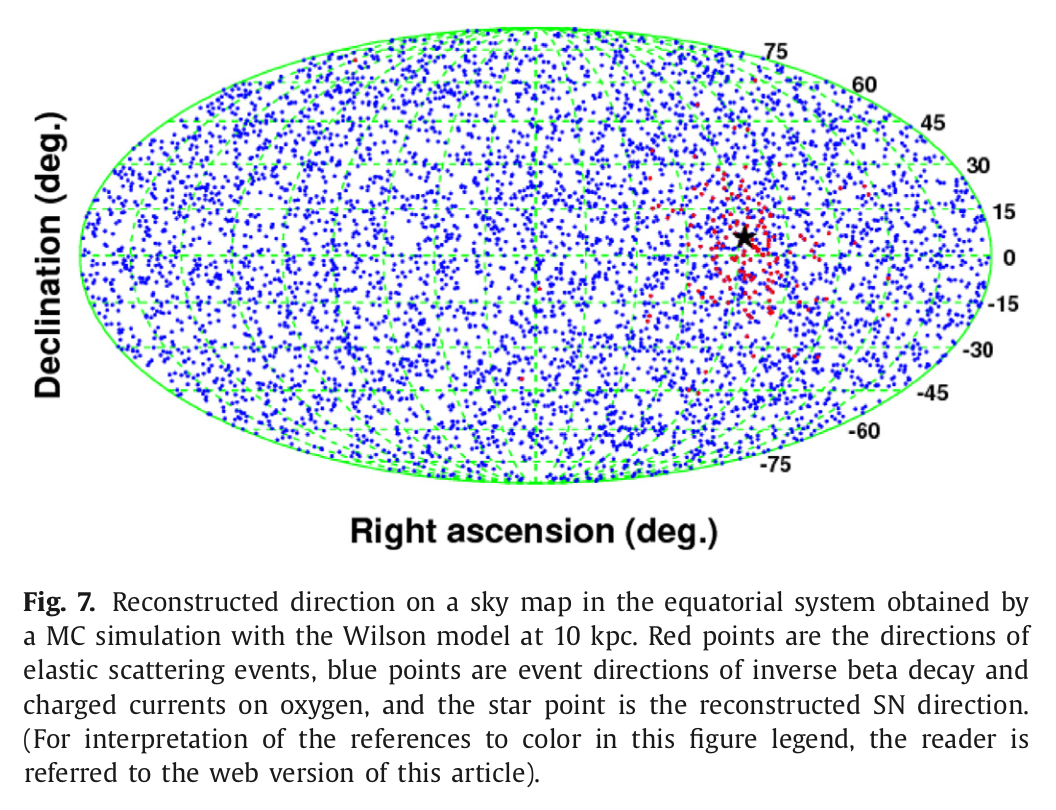
\includegraphics[width=4.0in]{SK-realtime-monitor-pointing}
    \caption{Caption... replace with real figure and no screen grab.}
    \label{fig:SK-realtime-monitor-pointing}
  \end{center}
\end{figure}

\begin{figure}
  \begin{center}
    \begin{minipage}[b]{3.1in}
      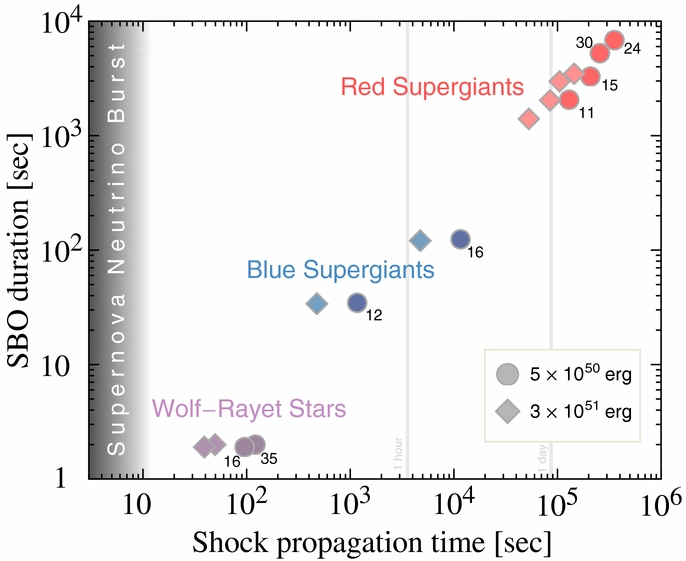
\includegraphics[width=3.0in]{apj487119f2_hr}
      \caption{Caption}
      \label{fig:delay-times}
    \end{minipage}
    \begin{minipage}[b]{3.1in}
      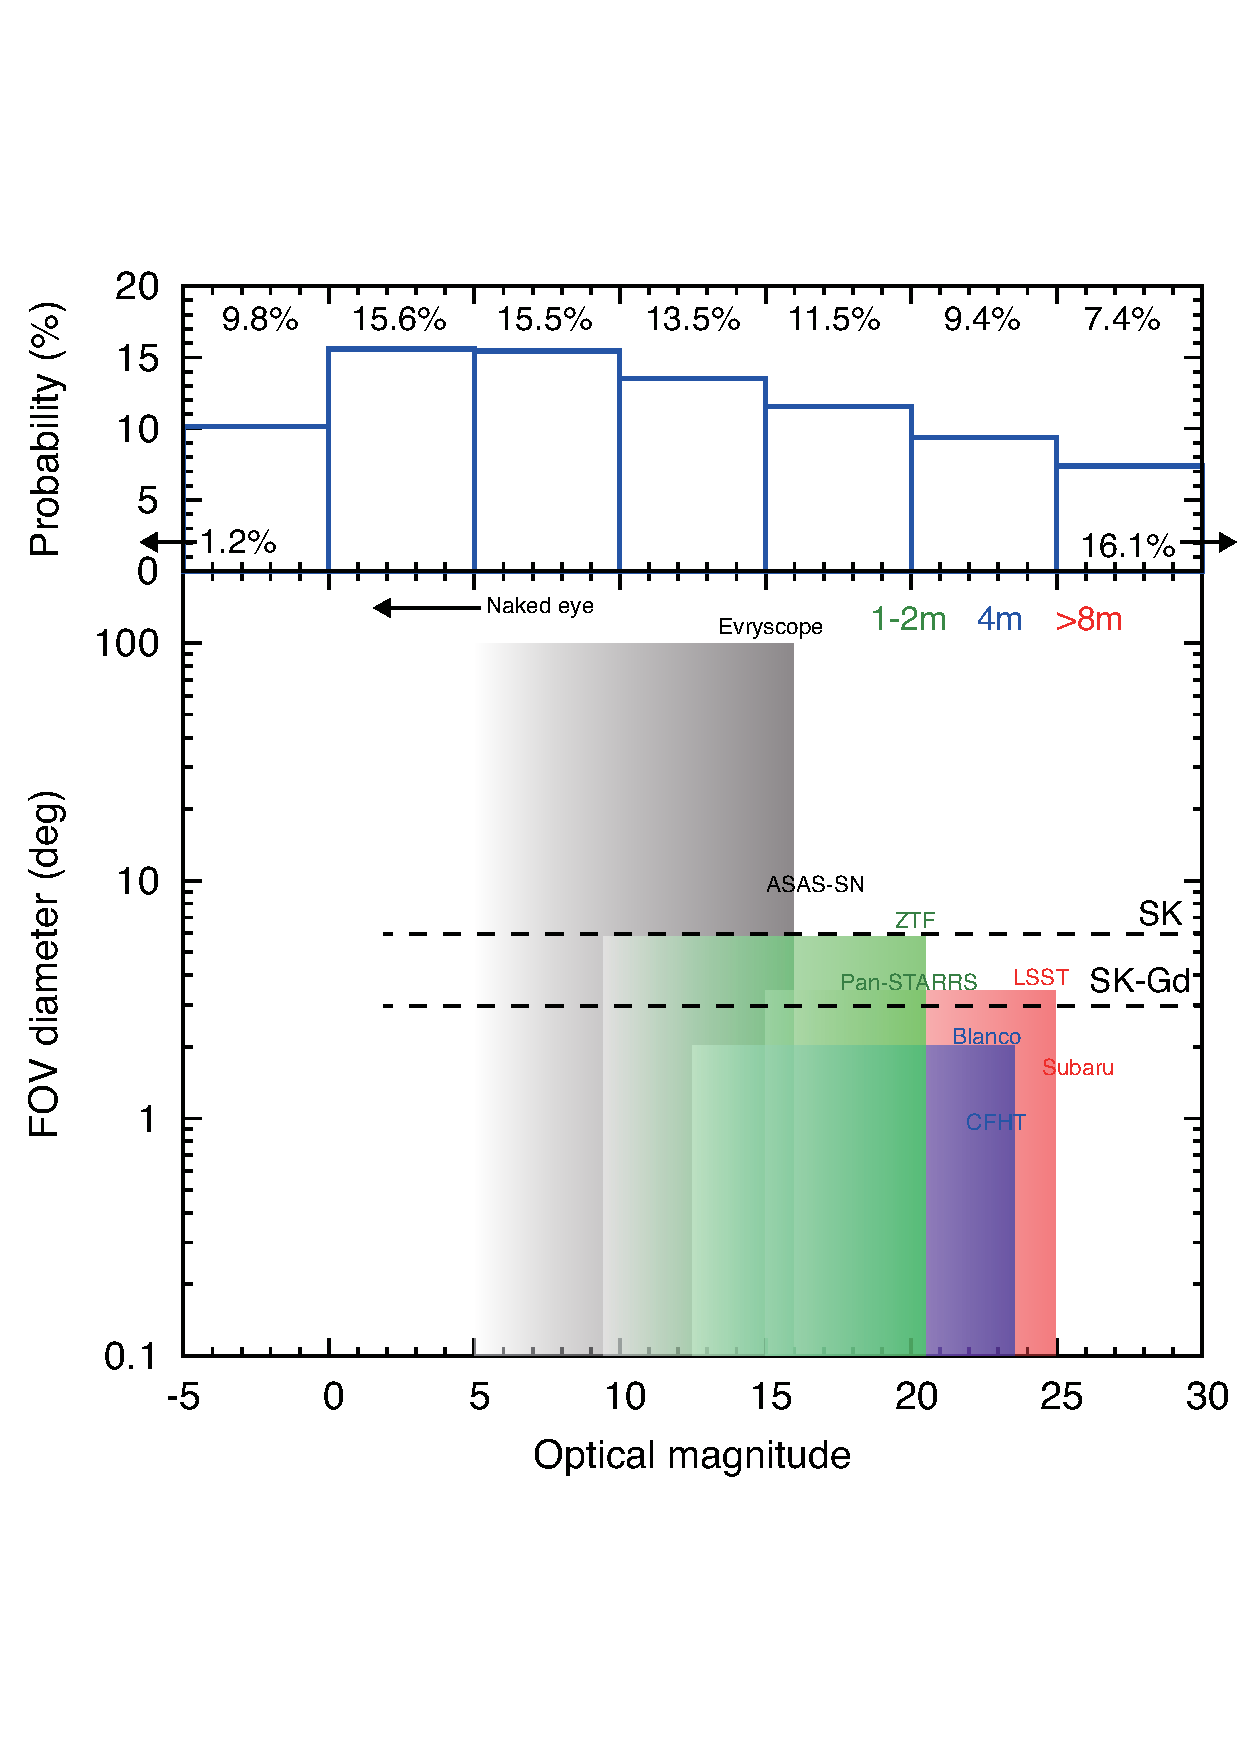
\includegraphics[width=3.0in]{fig9}
      \caption{Caption}
      \label{fig:multimessenger-comparison}
    \end{minipage}
  \end{center}
\end{figure}

\clearpage

\newpage
\section{Technical Description}
\begin{footnotesize}
{\it Describe your survey strategy modifications or proposed observations. Please comment on each observing constraint
below, including the technical motivation behind any constraints. Where relevant, indicate
if the constraint applies to all requested observations or a specific subset. Please note which 
constraints are not relevant or important for your science goals.}
\end{footnotesize}

In order to describe the survey strategy for footprint, tiling method,
depth, and observation frequency it is important to understand the
expected time delay and pointing signal and the form of the alarm signal.

\subsection{Expected Time Delay}

minutes WR - hours blue giant - ~day for red supergiant. Fill in with
info and link to paper / figure~\ref{fig:delay-times}.

\subsection{Expected pointing resolution}

The expected pointing resolution in a water Cherenkov detector will
scale with the number of interactions detected.  As explained in
section~\ref{sec:motivation} a set of electron scattering interactions which
point back to the supernova will be sitting on top of a background of
non-pointing interactions from the IBD neutrino captures.

For a supernova located 10kpc from the Earth (the galactic center is
approximately 8kpc away) the order of 10,000 neutrino interactions are
expected in \superk.  Supernova that are closer or further away will
have their fluxes scaled simply by scaling to their distance with a
factor of $1/r^2$.  Although 10,000 interactions are typical, expected
fluxes are found to have a range of values by different simulation
groups varying by factors of XXX~\cite{model_references}.  Given a
number of interactions, pointing to the supernova by fitting the
electron scattering signal on top of the IBD background is found to
give a resolution of approximately
%
$$ \Delta \theta = \frac{30^\circ}{\sqrt{N}.}, $$
%
where N is the number of electron-neutrino scattering interactions and
the angular resolution is a half-opening
angle~\cite{2012ARNPS..62...81S}.  With roughly 1\% of 10,000
interactions from a 10kpc supernova being electron scattering events,
this tells us that we should expect a rough pointing resolution of
$3^\circ$.  Closer supernova will have higher numbers of interactions
with better pointing, and those further away will have their
resolution decreased.

A more careful study by the \superk collaboration
in~\cite{2016APh....81...39A} plots a 68\% opening angle coverage as a
function of distance for a few flux
models. Figure~\ref{fig:SK-realtime-pointing-resolution} shows how the
pointing is expected to scale as a function of distance with neutrino
oscillations taken into account for one of the models. At 10kpc the
pointing is near $3^\circ$ as expected.

By the time the LSST survey begins we expect \superk to be doped with
0.02\% GdSo4.  The addition of gadolinium (which has a high neutron
cross-section) to the water will allow the neutron to be tagged in IBD
events thus removing a portion of the non-pointing background and
improving the pointing resolution. [Need more details? phases? Have
private plot from Nakahata...]

\begin{figure}
  \begin{center}
    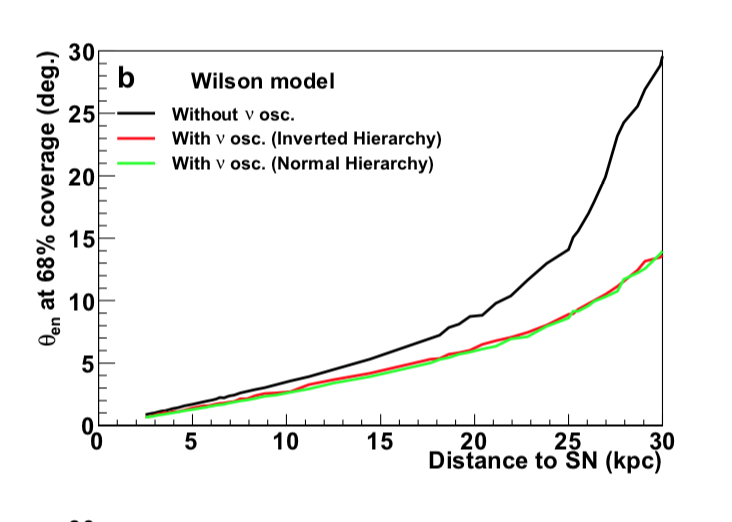
\includegraphics[width=3.0in]{SK-realtime-pointing-resolution}
    \caption{}
    \label{fig:SK-realtime-pointing-resolution}
  \end{center}
\end{figure}

\subsection{Alert input}

In order to point LSST, the observatory control system (OCS) must first
receive information from the neutrino experiments that a light from a
galactic supernova is about to arrive.  Time is of the essence since
depending on the size and type of the star the breakout time could
range from minutes to several hours~\cite{2013ApJ...778...81K}.  There
currently more than one way to receive an alert. If selected LSST must
work with the neutrino community to ensure that the proper information
that LSST needs is being promptly transferred.

There are two broad classes of alerts to consider.  Each experiment
has the option to send its own alert to the astronomical community.
For example, if \superk determines a CCSN in our galaxy has occurred
it might send the following template like text to the Astronomers
Telegram:


\begin{verbatim}
Super-Kamiokande, a 50000 ton water Cherenkov imaging detector
situated 1000 meters underground in the Kamioka mine, Gifu, Japan, has
observed a neutrino burst from a nearby supernova.  Within a fiducial
volume of 22500 tons, preliminary results indicate 5227
neutrino-produced events have been detected with energies greater than
7.0 MeV. An SN1987A-like explosion would be expected to produce such a
signal in Super-Kamiokande if the progenitor star was located at a
distance between 7.55 and 10.36 kpc from Earth. These events were
observed over an interval of 17.9 seconds, with the first event
arriving at 2017 Nov 2.318437 UT. The estimated supernova direction is
R.A. = 110 (degrees) and Dec.= 6 (degrees), within 3.29, 4.72 and 5.62
degrees for, respectively, 68, 90 and 95% C.L. error circles. 
The probability to have the SN located within 2, 5, and 10 degrees 
of the central position is 0.36, 0.92 and 1.00, respectively.
\end{verbatim}

C.W. Walter is a member of both \superk and the LSST project and
the \superk spokesperson has expressed interest in personal
conversation to supply direct information to the LSST OCS in whatever
form is most appropriate.

For many years the neutrino community as a whole has being preparing
for a galactic supernova through the creation of the Supernova Early
Warning System (SNEWS) SNEWS acts as a
broker and a blinded system to look for coincidences in time between
supernova alarms coming from different neutrino experiments. If one is
seen, then they alert the entire astronomical community through several
channels. This reduces the false coincidence rate to less than one
alert per century. SNEWS can also act as a broker passing alerts from
individual experiments to their alert system

SNEWS has several ways of making announcements to the community.  They
also give a direct connection to the IceCube experiment which benefits
from an external trigger.  A direct connection to LSST could also be
arranged.  Current  alerts include announcements to the GCN (a
template is seen below):

% SNEWS template
\begin{verbatim}
TITLE:         GCN/SNEWS EVENT NOTICE
NOTICE_DATE:   Tue 26 Jun 18 16:00:08 UT
NOTICE_TYPE:   TEST COINCIDENCE
TRIGGER_NUM:   1000182
EVENT_RA:      Undefined (J2000),
              Undefined (current),
              Undefined (1950)
EVENT_DEC:     Undefined (J2000),
              Undefined (current),
              Undefined (1950)
EVENT_ERROR:   360.0 [deg radius, statistical plus systematic], 68.00% containment
EVENT_FLUENCE: 0 [neutrinos]
EVENT_TIME:    57601.00 SOD {16:00:01.00} UT
EVENT_DATE:    18295 TJD;   177 DOY;   18/06/26
EVENT_DUR:     0.00 [sec]
EXPT:          Detector_A Good, Detector_B Good, Detector_D Possible, Detector_E Good, Detector_F Possible, 
SUN_POSTN:      95.45d {+06h 21m 49s}  +23.34d {+23d 20' 30"}
SUN_DIST:      Undefined [deg]
MOON_POSTN:    257.26d {+17h 09m 02s}  -19.06d {-19d 03' 38"}
MOON_DIST:     Undefined [deg]
MOON_ILLUM:    98 [%]
GAL_COORDS:    Undefined,Undefined [deg] galactic lon,lat of the event
ECL_COORDS:    Undefined,Undefined [deg] ecliptic lon,lat of the event
COMMENTS:      SNEWS Event without RA,Dec coordinates.  
COMMENTS:      This is a Test COINCIDENCE notice.  It is NOT a Real event.  
COMMENTS:      This is a Test COINCIDENCE notice.  The EXPT labels have been anonymized.  
COMMENTS:         
COMMENTS:      RA,Dec fields undefined.  
COMMENTS:      For more information see:  
COMMENTS:
\end{verbatim}

% SNEWS direct template

\noindent
and email alerts such as the template below.

\begin{verbatim}
-----BEGIN PGP SIGNED MESSAGE-----
Hash: SHA1

- ---------------------------------------------
*** SNEWS ALERT ***
Coincidence rating: GOLD
Alarms in the coincidence:
Experiment: 5 LVD
Level: GOOD
Time: Jan 02 2006 22:34:37.000000000
Duration:   10.00
No. of signal events:    0.00
Right Ascension:    0.00
Declination:    0.00
Error:  360.10
- ---------------------------------------------
Experiment: 3 SNO
Level: GOOD 
Time: Jan 02 2006 22:34:37.000000000
Duration:   10.00
No. of signal events:    0.00
Right Ascension:    0.00
Declination:    0.00
Error:  360.10
- ---------------------------------------------
Experiment: 1 Super-K
Level: POSSIBLE 
Time: Jan 02 2006 22:34:37.000000000
Duration:   10.00
No. of signal events:    0.00
Right Ascension:    13.00
Declination:    -3.00
Error:  4.0
- ---------------------------------------------

For information, see web page http://snews.bnl.gov/
-----BEGIN PGP SIGNATURE-----
Version: GnuPG v1.4.9 (GNU/Linux)

iD8DBQFMhguY4A2qNGjfk/cRAp+DAKD2cFdN4aHZomU87XhhA2r7GalWcACgt/oM
ffObwWjd44FA6kx5gx/RLDQ=
=DtVE
-----END PGP SIGNATURE-----
\end{verbatim}

Currently, a fast alarm goes directly from \superk to the SNEWS system
with no human intervention.  However, that alarm does not contain
pointing information.  Now, that information is released only after a
virtual meeting of \superk collaborators to confirm the alarm.
However, it is recognized that this step slows down dissemination, so
discussion is starting on the best way to pass this information either
directly to projects like LSST or through systems like SNEWS.

LSST could decide to require multiple or single experimental alarms
still taking the pointing system from \superk.  In the future, SNEWS
is also expected to supply pointing based on triangulation using
timing and this information could be combined with the electron
scattering signal.

\subsection{High-level description}
\begin{footnotesize}
{\it Describe or illustrate your ideal sequence of observations.}
\end{footnotesize}

\vspace{.3in}


Describe sequence here:

\begin{itemize}
\item Receive alert
\item Go into SN watch mode
\item choose exposure, filter and dither pattern
\item Perform fast DIA analysis to locate CCSN candidate
\item Pass information about the CCSN candidate to community o allow
  other followup observations.
\item Follow for some time for the rest of the night of observation.
\end{itemize}

\subsection{Footprint -- pointings, regions and/or constraints}
\begin{footnotesize}{\it Describe the specific pointings or general region (RA/Dec, Galactic longitude/latitude or 
Ecliptic longitude/latitude) for the observations. Please describe any additional requirements, especially if there
are no specific constraints on the pointings (e.g. stellar density, galactic dust extinction).}
\end{footnotesize}

Depending on the pointing resolution the OCS would either point the
telescope at one point in the sky taking a continuous set of
exposures, or likely put it in a tight dither pattern covering a few
FOVs worth of area.

\subsection{Image quality}
\begin{footnotesize}{\it Constraints on the image quality (seeing).}\end{footnotesize}

The image quality is not relevant.

\subsection{Individual image depth and/or sky brightness}
\begin{footnotesize}{\it Constraints on the sky brightness in each image and/or individual image depth for point sources.
Please differentiate between motivation for a desired sky brightness or individual image depth (as 
calculated for point sources). Please provide sky brightness or image depth constraints per filter.}
\end{footnotesize}

Not relevant.

\subsection{Co-added image depth and/or total number of visits}
\begin{footnotesize}{\it  Constraints on the total co-added depth and/or total number of visits.
Please differentiate between motivations for a given co-added depth and total number of visits. 
Please provide desired co-added depth and/or total number of visits per filter, if relevant.}
\end{footnotesize}

Not relevant (?).  Should we try to build a co-add?

\subsection{Number of visits within a night}
\begin{footnotesize}{\it Constraints on the number of exposures (or visits) in a night, especially if considering sequences of visits.  }
\end{footnotesize}

This mode would be envisioned to completely take over the facility for
one dark period after the alarm arrives.

\subsection{Distribution of visits over time}
\begin{footnotesize}{\it Constraints on the timing of visits --- within a night, between nights, between seasons or
between years (which could be relevant for rolling cadence choices in the WideFastDeep. 
Please describe optimum visit timing as well as acceptable limits on visit timing, and options in
case of missed visits (due to weather, etc.). If this timing should include particular sequences
of filters, please describe.}
\end{footnotesize}

Note relevant.

\subsection{Filter choice}
\begin{footnotesize}
{\it Please describe any filter constraints not included above.}
\end{footnotesize}

Peak height vs NIR for seeing through dust. Need to look at light
curves and throughput.

\subsection{Exposure constraints}
\begin{footnotesize}
{\it Describe any constraints on the minimum or maximum exposure time per visit required (or alternatively, saturation limits).
Please comment on any constraints on the number of exposures in a visit.}
\end{footnotesize}

Dynamic exposure? What happens if it is too bright?


\subsection{Other constraints}
\begin{footnotesize}
{\it Any other constraints.}
\end{footnotesize}

\subsection{Estimated time requirement}
\begin{footnotesize}
{\it Approximate total time requested for these observations, using the guidelines available at \url{https://github.com/lsst-pst/survey_strategy_wp}.}
\end{footnotesize}

We expect no more than one night in the 10 year survey would be
affected by this program. With an expected rate of 3 per century there
is a 22\% chance one CCSN would be seen and a 3\% chance there could
be two.

\vspace{.3in}

\begin{table}[ht]
    \centering
    \begin{tabular}{l|l|l|l}
        \toprule
        Properties & Importance \hspace{.3in} \\
        \midrule
        Image quality &     \\
        Sky brightness &  \\
        Individual image depth &   \\
        Co-added image depth &   \\
        Number of exposures in a visit   &   \\
        Number of visits (in a night)  &   \\ 
        Total number of visits &   \\
        Time between visits (in a night) &  \\
        Time between visits (between nights)  &   \\
        Long-term gaps between visits & \\
        Other (please add other constraints as needed) & \\
        \bottomrule
    \end{tabular}
    \caption{{\bf Constraint Rankings:} Summary of the relative importance of various survey strategy constraints. Please rank the importance of each of these considerations, from 1=very important, 2=somewhat important, 3=not important. If a given constraint depends on other parameters in the table, but these other parameters are not important in themselves, please only mark the final constraint as important. For example, individual image depth depends on image quality, sky brightness, and number of exposures in a visit; if your science depends on the individual image depth but not directly on the other parameters, individual image depth would be `1' and the other parameters could be marked as `3', giving us the most flexibility when determining the composition of a visit, for example.}
        \label{tab:obs_constraints}
\end{table}

\subsection{Technical trades}
\begin{footnotesize}
{\it To aid in attempts to combine this proposed survey modification with others, please address the following questions:
\begin{enumerate}
    \item What is the effect of a trade-off between your requested survey footprint (area) and requested co-added depth or number of visits?
    \item If not requesting a specific timing of visits, what is the effect of a trade-off between the uniformity of observations and the frequency of observations in time? e.g. a `rolling cadence' increases the frequency of visits during a short time period at the cost of fewer visits the rest of the time, making the overall sampling less uniform.
    \item What is the effect of a trade-off on the exposure time and number of visits (e.g. increasing the individual image depth but decreasing the overall number of visits)?
    \item What is the effect of a trade-off between uniformity in number of visits and co-added depth? Is there any benefit to real-time exposure time optimization to obtain nearly constant single-visit limiting depth?
    \item Are there any other potential trade-offs to consider when attempting to balance this proposal with others which may have similar but slightly different requests?
\end{enumerate}}
\end{footnotesize}

Not relevant.

\section{Performance Evaluation}
\begin{footnotesize}
{\it Please describe how to evaluate the performance of a given survey in achieving your desired
science goals, ideally as a heuristic tied directly to the observing strategy (e.g. number of visits obtained
within a window of time with a specified set of filters) with a clear link to the resulting effect on science.
More complex metrics which more directly evaluate science output (e.g. number of eclipsing binaries successfully
identified as a result of a given survey) are also encouraged, preferably as a secondary metric.
If possible, provide threshold values for these metrics at which point your proposed science would be unsuccessful 
and where it reaches an ideal goal, or explain why this is not possible to quantify. While not necessary, 
if you have already transformed this into a MAF metric, please add a link to the code (or a PR to 
\href{https://github.com/lsst-nonproject/sims_maf_contrib}{sims\_maf\_contrib}) in addition to the text description. (Limit: 2 pages).}
\end{footnotesize}

Not relevant.  Performance would be measured in successfully
identifying and quickly notifying the community of the location of the
optical supernova counterpart.


\vspace{.6in}

\section{Special Data Processing}
\begin{footnotesize}
{\it Describe any data processing requirements beyond the standard LSST Data Management pipelines and how these will be achieved.}
\end{footnotesize}

A version of the DIA pipeline would need to be utilized to make the
initial identification.

\section{References}
% Shared ADS library: https://ui.adsabs.harvard.edu/#/public-libraries/tD3_JEzETqaCHFp83Dk74g

\bibliographystyle{hunsrt} 
\bibliography{references}

\end{document}
